\chapter{Design}
\label{chap:design}
As the project has utilised an iterative
approach with the Kanban methodology, the design has changed and been refined
throughout the project. The design of the software will be broken down into 3
sections, namely the design of the web application and the design of the \gls{aci}
and vCenter configuration.
The design of the testbed will also be detailed.

\section{Web Application}
\label{design:web-application}
\subsection{Architecture}
\label{design:web-application:architecture}

A client-server architecture will be utilised to provide the user-facing
experience and the automation and data handling logic will be hosted on the server. By
using this model, many clients can request and interact with data that is
hosted on one central server. The back-end and front-end that make up the
application will be separate from one another, and will therefore be developed
independently, with the front-end interacting with the back-end via a \gls{rest} \gls{api}.
This allows for the front-end to be an \gls{spa}, which facilitates a better user
experience due to the lack of page refreshes upon every request.

The server
will process all requests generated by the front end and also make requests to
the various \gls{api}s that will be required to automate the network deployment. The database will also store all data required by the server to generate the
appropriate \gls{aci} and network configuration that is required to automate the deployment
of projects to the \gls{aci} fabric and associated network devices.

\begin{figure}[H]
    \centering

    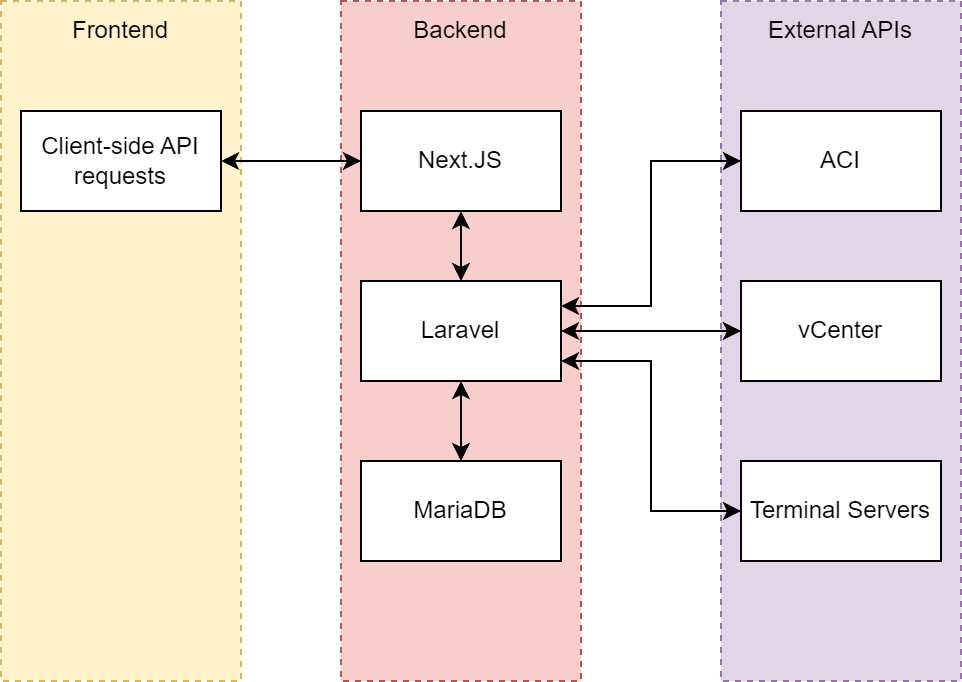
\includegraphics[scale=0.3]{images/web-architecture.png}
    \caption{Web
        Architecture Design}
    \label{fig:web-architecture}
\end{figure}

\subsection{Front-end}
\label{design:web-application:front-end}
Next.js will be
used to power the front-end of the application as it is an enhancement of
React.js and provides server-side rendering and acceleration of pages. React
uses a modular 'componentised' approach to building front-end user interfaces, which allows
for the creation of reusable components that can be used throughout the
application. This allows for the creation of a modular and scalable front-end
that can be easily extended and maintained.

React.js also has an extensive
library of open-source components and libraries that can be utilised to make
developing the front-end easier and more feature-complete. Due to the complexity
of some required features, such as having a drag-and-drop interface for the
recreation of the lab space, the use of a library such as React Flow will be
required as the time required to develop such a feature would be out of the
scope of this project.

Tailwind CSS and Flowbite will be used to style the web application. Tailwind CSS allows for the creation of custom components and styles that can be reused throughout the application. Flowbite is a UI toolkit that is built on top of Tailwind CSS and provides a set of pre-built components that can be used to accelerate the development process. Tailwind CSS also provides features such as native support for dark mode, which is a feature that is becoming more popular in modern applications.

\subsection{Back-end}
\label{design:web-application:back-end}
The back end of the application will be
written in PHP, using the Laravel PHP framework. Laravel is a popular PHP
framework that will accelerate the development process as it features an
inbuilt \gls{orm}, \gls{api} routing system and an authentication system that
can be implemented. Laravel utilises SQL-based databases, and as such MariaDB
will be used as the database for the application. Laravel also features an
in-built \gls{http} client which will be required to interact with the
\gls{aci} and vCenter \gls{api}s which are all \gls{rest}-based.

Laravel
follows the \gls{mvc} architecture, however as the front-end is a React
\gls{spa}, Laravel will only be used to provide and consume the data via its
\gls{rest} \gls{api}.

Laravel also features a queuing system which allows for jobs to be processes asynchronously without affecting the process responsible for handling \gls{api} calls from the web interface.

\subsection{Database Design}
\label{design:web-application:database}
As the project will need to store data
persistently, ensuring that the database has an appropriately designed schema
will ensure that the data is stored in a way that is easily accessible and can
be queried efficiently. The design of the database was tweaked and refined
throughout the development process, however, the final \gls{erd} is shown below
in figure \ref{fig:database-erd}.

\begin{figure}[H]
    \centering

    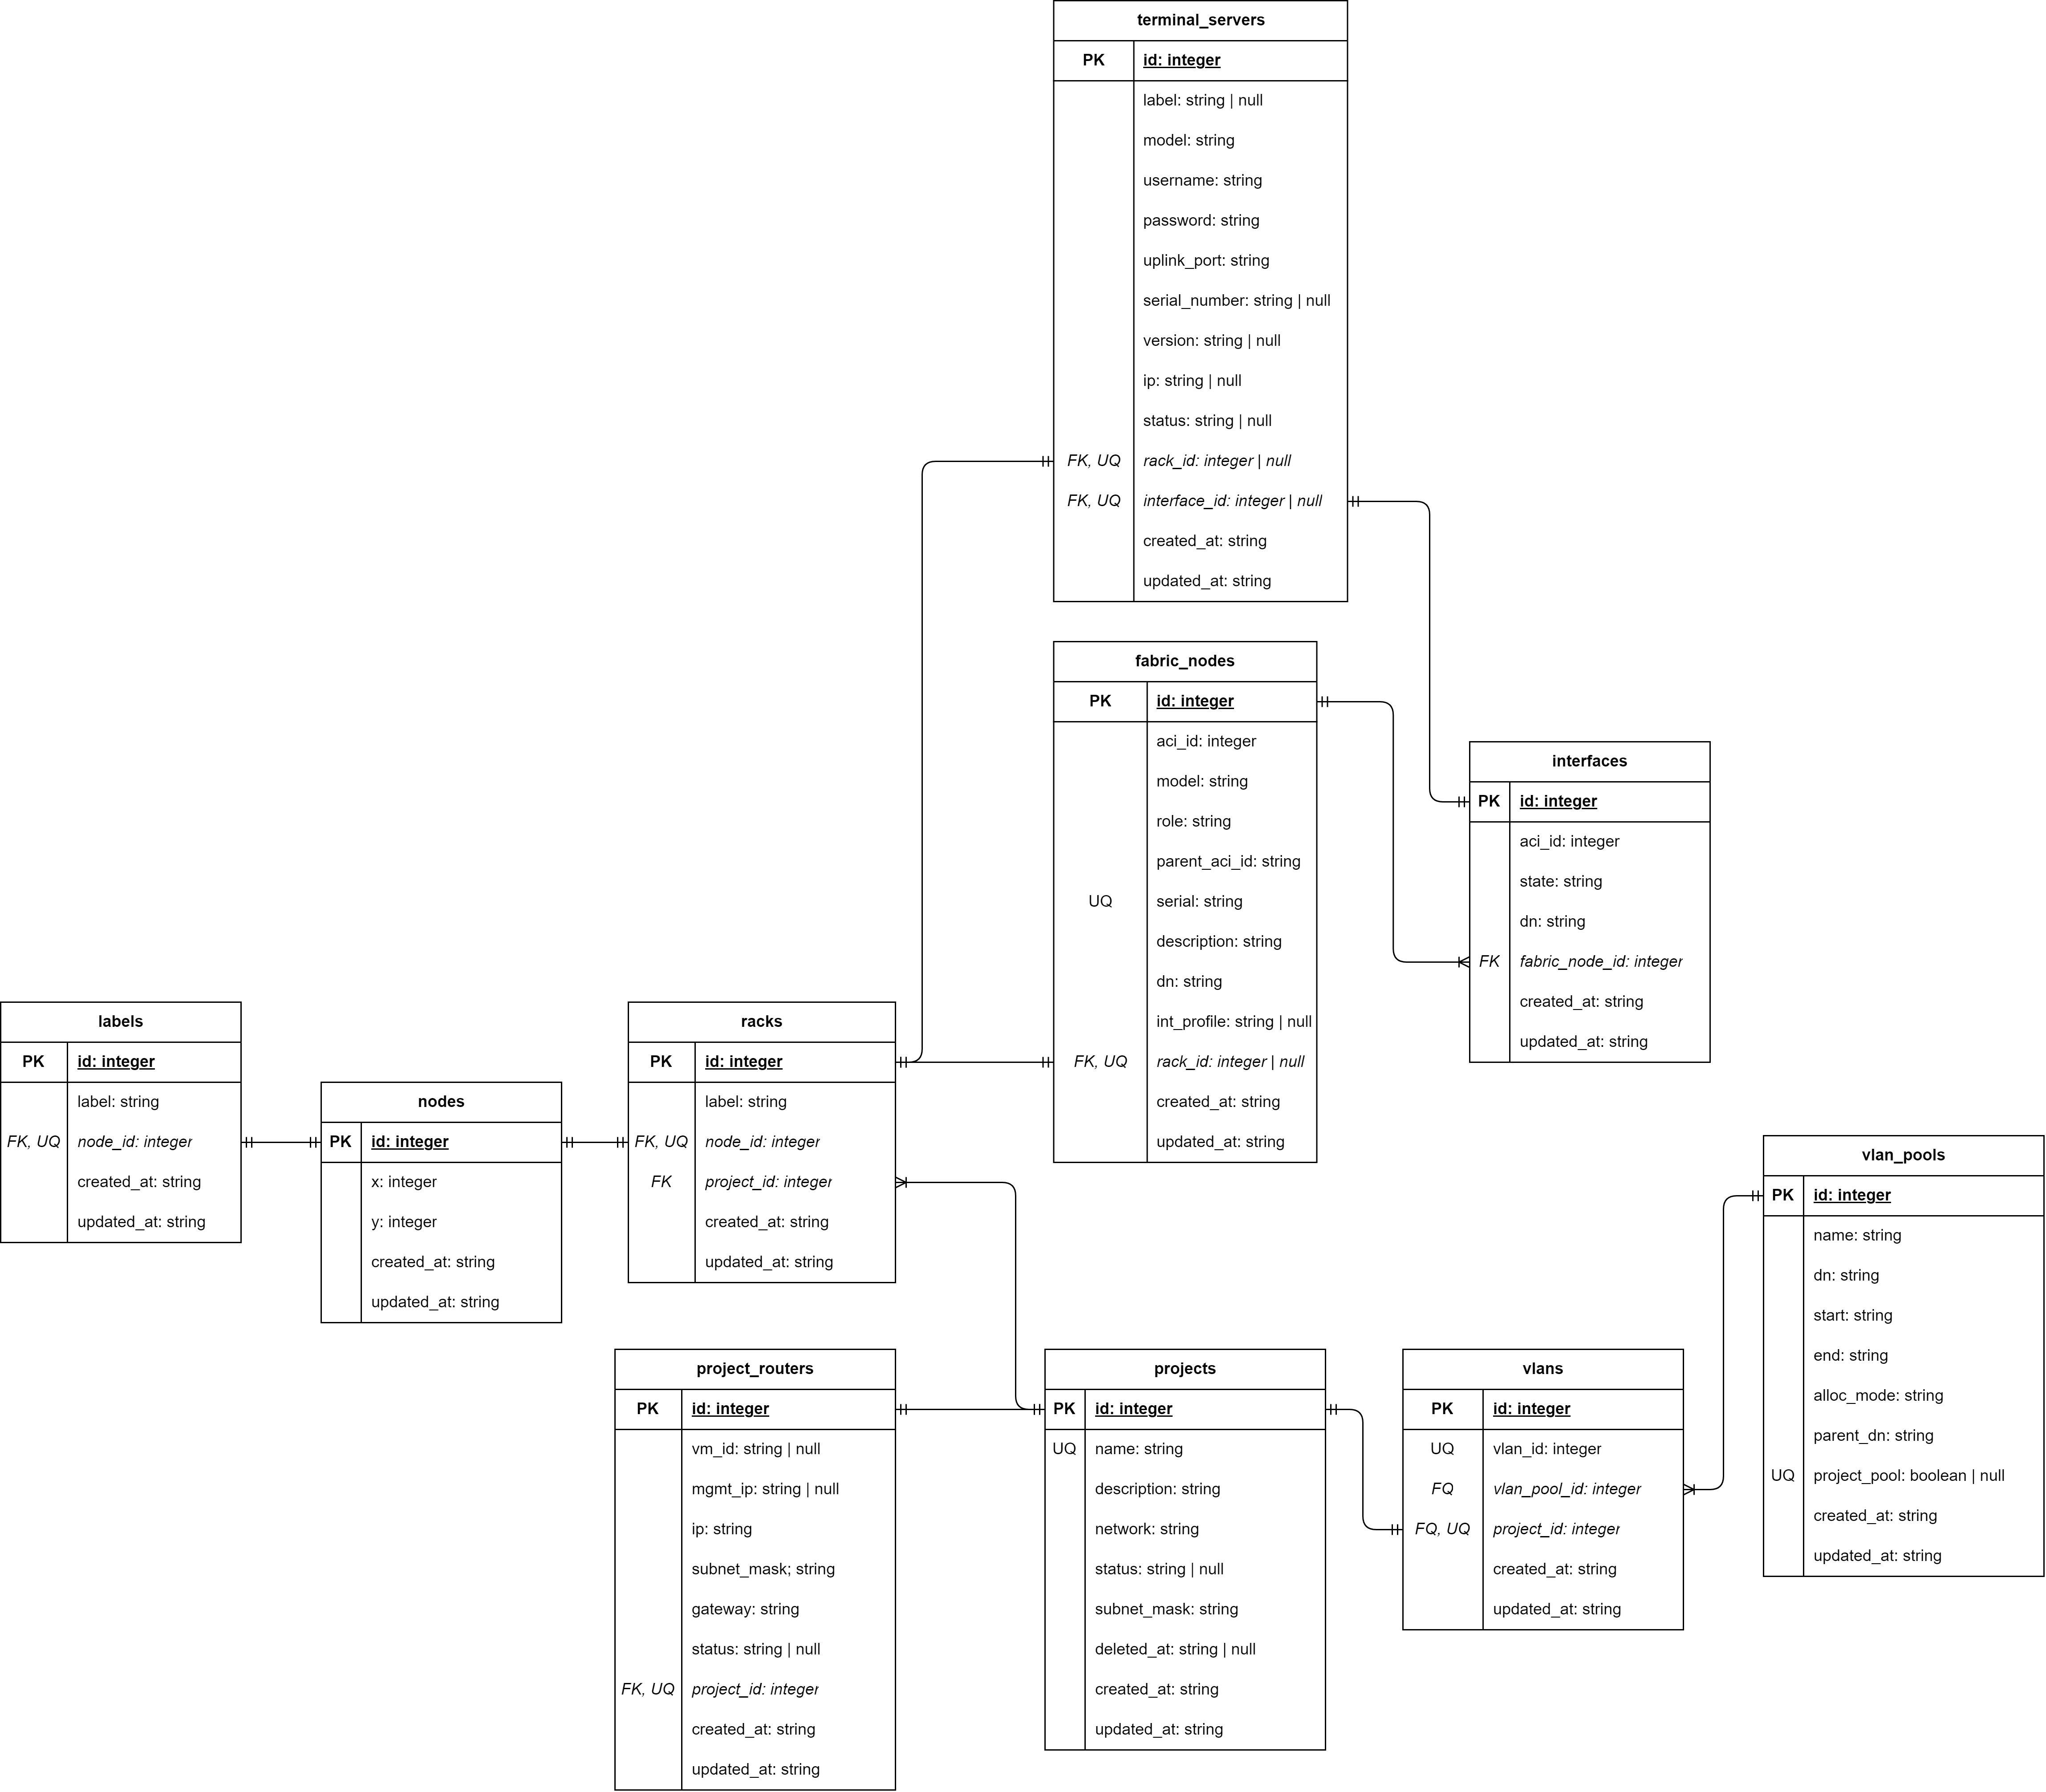
\includegraphics[scale=0.1]{images/erd.png}
    \caption{Database ERD}

    \label{fig:database-erd}
\end{figure}

\subsubsection{Nodes}
\label{design:web-application:database:nodes}
Nodes provide the root of storing
information about the layout of the rack space. Each node can either have a rack
or a label attached to it. Labels will serve as a place to store text
information on the rack space diagram for informational purposes only. Racks
will represent a physical rack in the rack space. By using a node table, the
position of the node can be abstracted away from the other data which is more
relevant to the automation functionality of the solution. A more refined and efficient query is also
possible as all nodes can be easily retrieved by selecting all nodes and then
joining the rack and label tables to retrieve the relevant information.

\subsubsection{Fabric Nodes and Interfaces}
\label{design:web-application:database:fabric-nodes-and-interfaces}
The fabric
nodes and interfaces tables will be used to store information related to all
fabric nodes that are attached to \gls{aci}. The tables will be populated by the automation script which will retrieve information about the
nodes and their associated interfaces from \gls{aci}. Each interface will tie
to a fabric node so that all interfaces belonging to a fabric node can be
easily retrieved. A Role and Parent ID field are also included in the fabric
node table which allows for \gls{fex}s to also be stored as nodes. \gls{aci}
treats \gls{fex}s as child nodes to leafs, hence why the Parent ID and role
field are needed to provide the correct differentiation between the two.

\subsubsection{Terminal Servers}
\label{design:web-application:database:terminal-servers}
The terminal servers
table will store information about the various terminal servers present in the
rack space - these will be inserted manually via the web UI. A relation will
also exist that associates an interface to a terminal server so that the
automation scripts can appropriately configure the uplink ports on the
\gls{aci} fabric.

\subsubsection{Projects}
\label{design:web-application:database:projects}
The projects table will store
all projects present in the application. Each project will link to the racks
via a Project ID field in the racks table. The project's private subnet will
also be stored with the project.

\subsubsection{Project Routers}
\label{design:web-application:database:project-routers}
A project router will
have a one-to-one relationship with a project, allowing only one project router
per project. This table will keep track of the virtual router that is created
for each project, and will also store the WAN IP address assigned to the
router.

\subsubsection{VLANs and VLAN Pool}
\label{design:web-application:database:vlan-and-vlan-pool}
The VLAN pool table
will store a list of all VLAN pools present in \gls{aci}. It will also store
the selection that the user has made as to the VLAN pool that should be used by
the automation platform for its endpoint groups. The VLANs table will be used
to keep a record of which project is using which VLAN within a VLAN pool so
that a VLAN cannot be used more than once.

\section{Testbed}
\label{design:Testbed}
To support the development of the automation platform,
it is necessary to have a network that can be used to test the automation
functionality on real hardware and software that would be used in production.
The network will be built using a scaled-down version of what could be deployed
in a real scenario; the same also applies to the associated compute and storage
resources.

\subsection{OOB Network}
\label{design:Testbed:network-design:oob}
To provide connectivity for management and day-zero configuration, it is
important to have a reliable \gls{oob} network. The purpose of an \gls{oob}
network is to provide access to networking and infrastructure equipment in a manner that is external
to the main network so that in the event of a failure, the devices can still be
reached to rectify any problem that may have occurred. The \gls{oob} network
will be a single Layer 2 network, with a single switch providing connectivity
to all devices. The switch will be a Cisco Catalyst 2960-XR, and will be
connected to external infrastructure which will host a \gls{vpn} server and a
\gls{nat} router so that devices connected to the \gls{oob} network also have
access to the internet, and accessible via the \gls{vpn}. The \gls{vm}s hosted on the ESXi server are also
detailed in the topology shown in figure \ref{fig:oob-topology}

\begin{figure}[H]
    \centering

    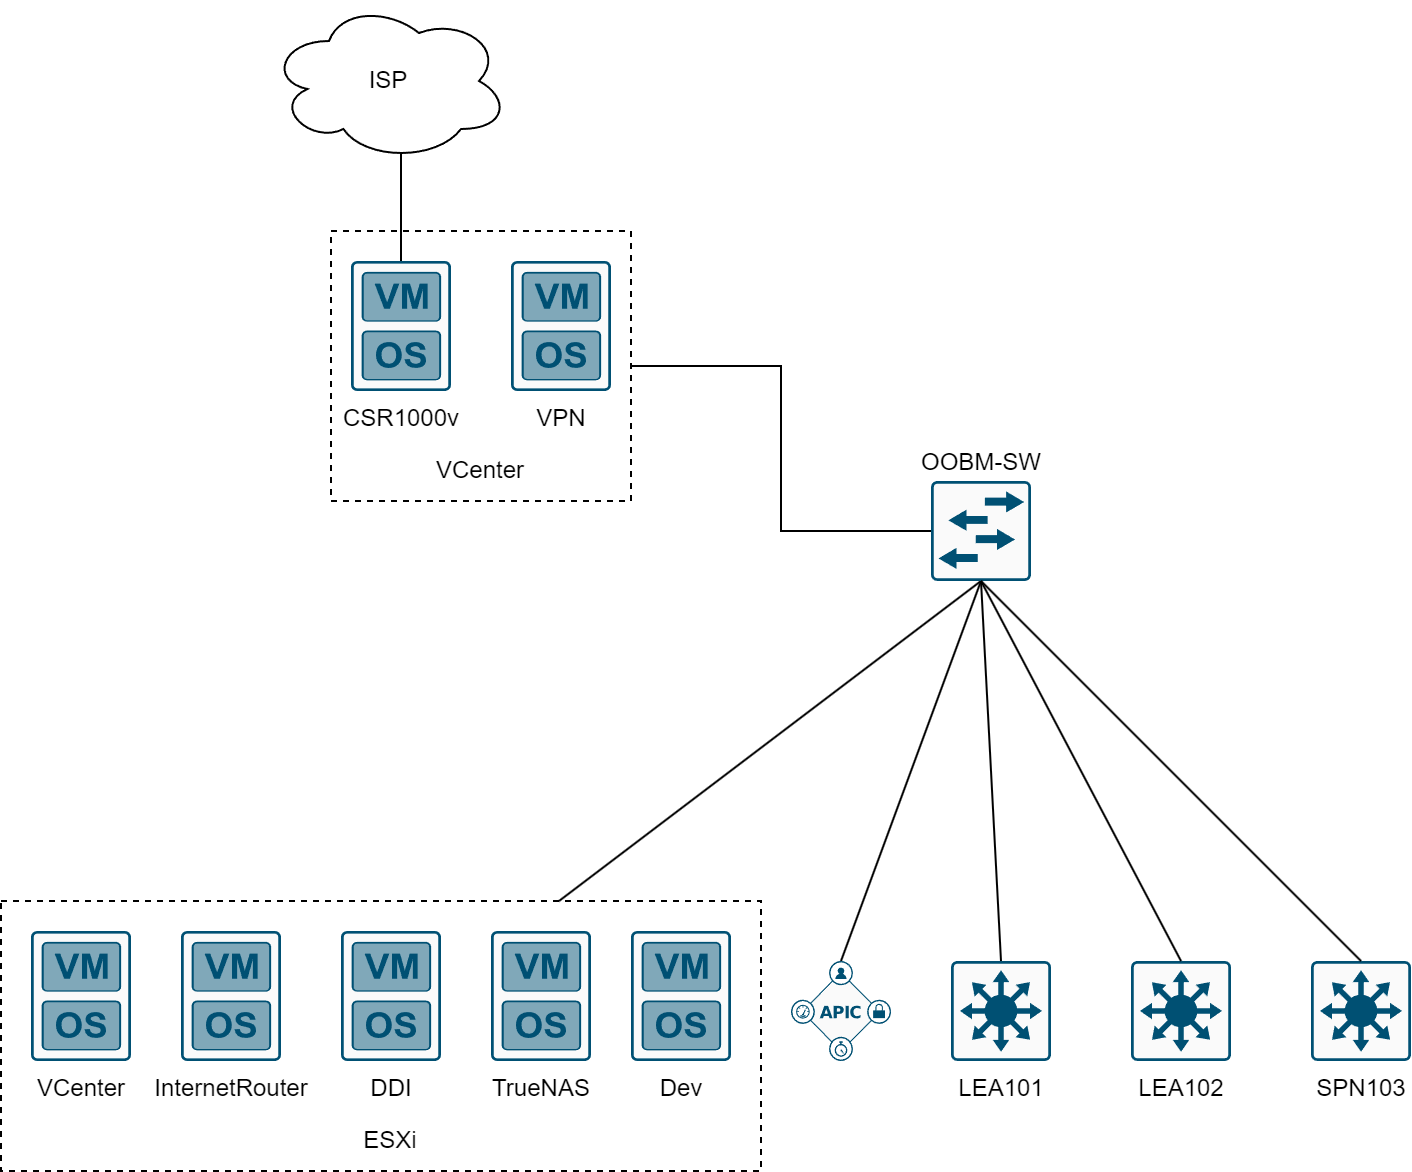
\includegraphics[scale=0.25]{images/oob-topology.png}
    \caption{OOB
        Topology}
    \label{fig:oob-topology}
\end{figure}

\subsection{ACI Fabric}
\label{design:Testbed:network-design}
As the automation platform is designed to
automate \gls{aci} fabrics, a reduced \gls{aci} fabric will be deployed for
development and testing. The base fabric will consist of one spine and two
leafs, these being the N9K-C9336PQ and N9K-C93180YC-EX respectively. The leafs
will also have a total of 3 \gls{fex}s attached to provide RJ45 connectivity to
the fabric and to also ensure that the automation platform will correctly
support FEXs. The FEXs used will be the N2K-C2248TP-E-1GE. \gls{aci} also
requires at least one \gls{apic} to function, so a single \gls{apic} M2 will be
connected to the pair of leafs to provide overall administration and control
over the fabric.

A single ESXi host will also be included in the network,
which will also be dual-homed to both leafs to provide connectivity and
test \gls{lacp} functionality. The ESXi host will be used to host the automation
platform and will also host the associated infrastructure required for the
automation platform to function, such as vCenter.

Two routers simulating
terminal servers will also be included in the design. Cisco routers can have
additional modules inserted into them allowing them to provide console
connectivity to devices via \gls{ssh} or Telnet.
Shown in figure
\ref{fig:fabric-topology} is the fabric topology that will be used for the
testbed. Device names/hostnames are shown in the figure for clarity.

\begin{figure}[H]
    \centering

    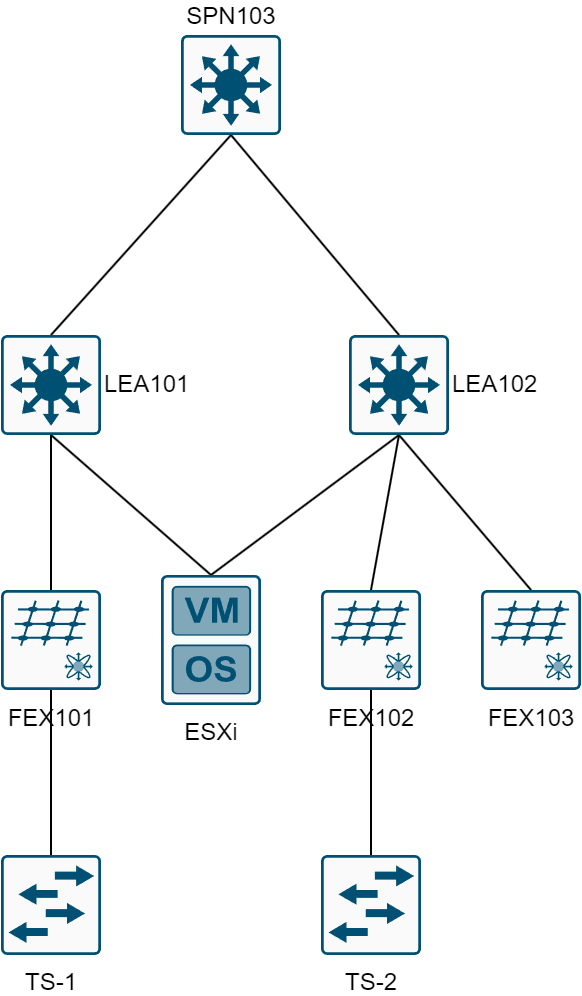
\includegraphics[scale=0.3]{images/aci-topology.png}
    \caption{Fabric
        Topology}
    \label{fig:fabric-topology}
\end{figure}

\subsection{ACI Policy}
\label{design:Testbed:network-design:aci-policy}
To provide internal
connectivity within the \gls{aci} testbed, the correct policy will need to be
designed to facilitate this. As \gls{aci} is policy-based, conventional
networking paradigms are shifted and abstracted behind \gls{aci}. Figure
\ref{fig:epg-topology} shows the tenant and the policy it houses that will be
created to provide connectivity within the testbed.

\begin{figure}[H]

    \centering
    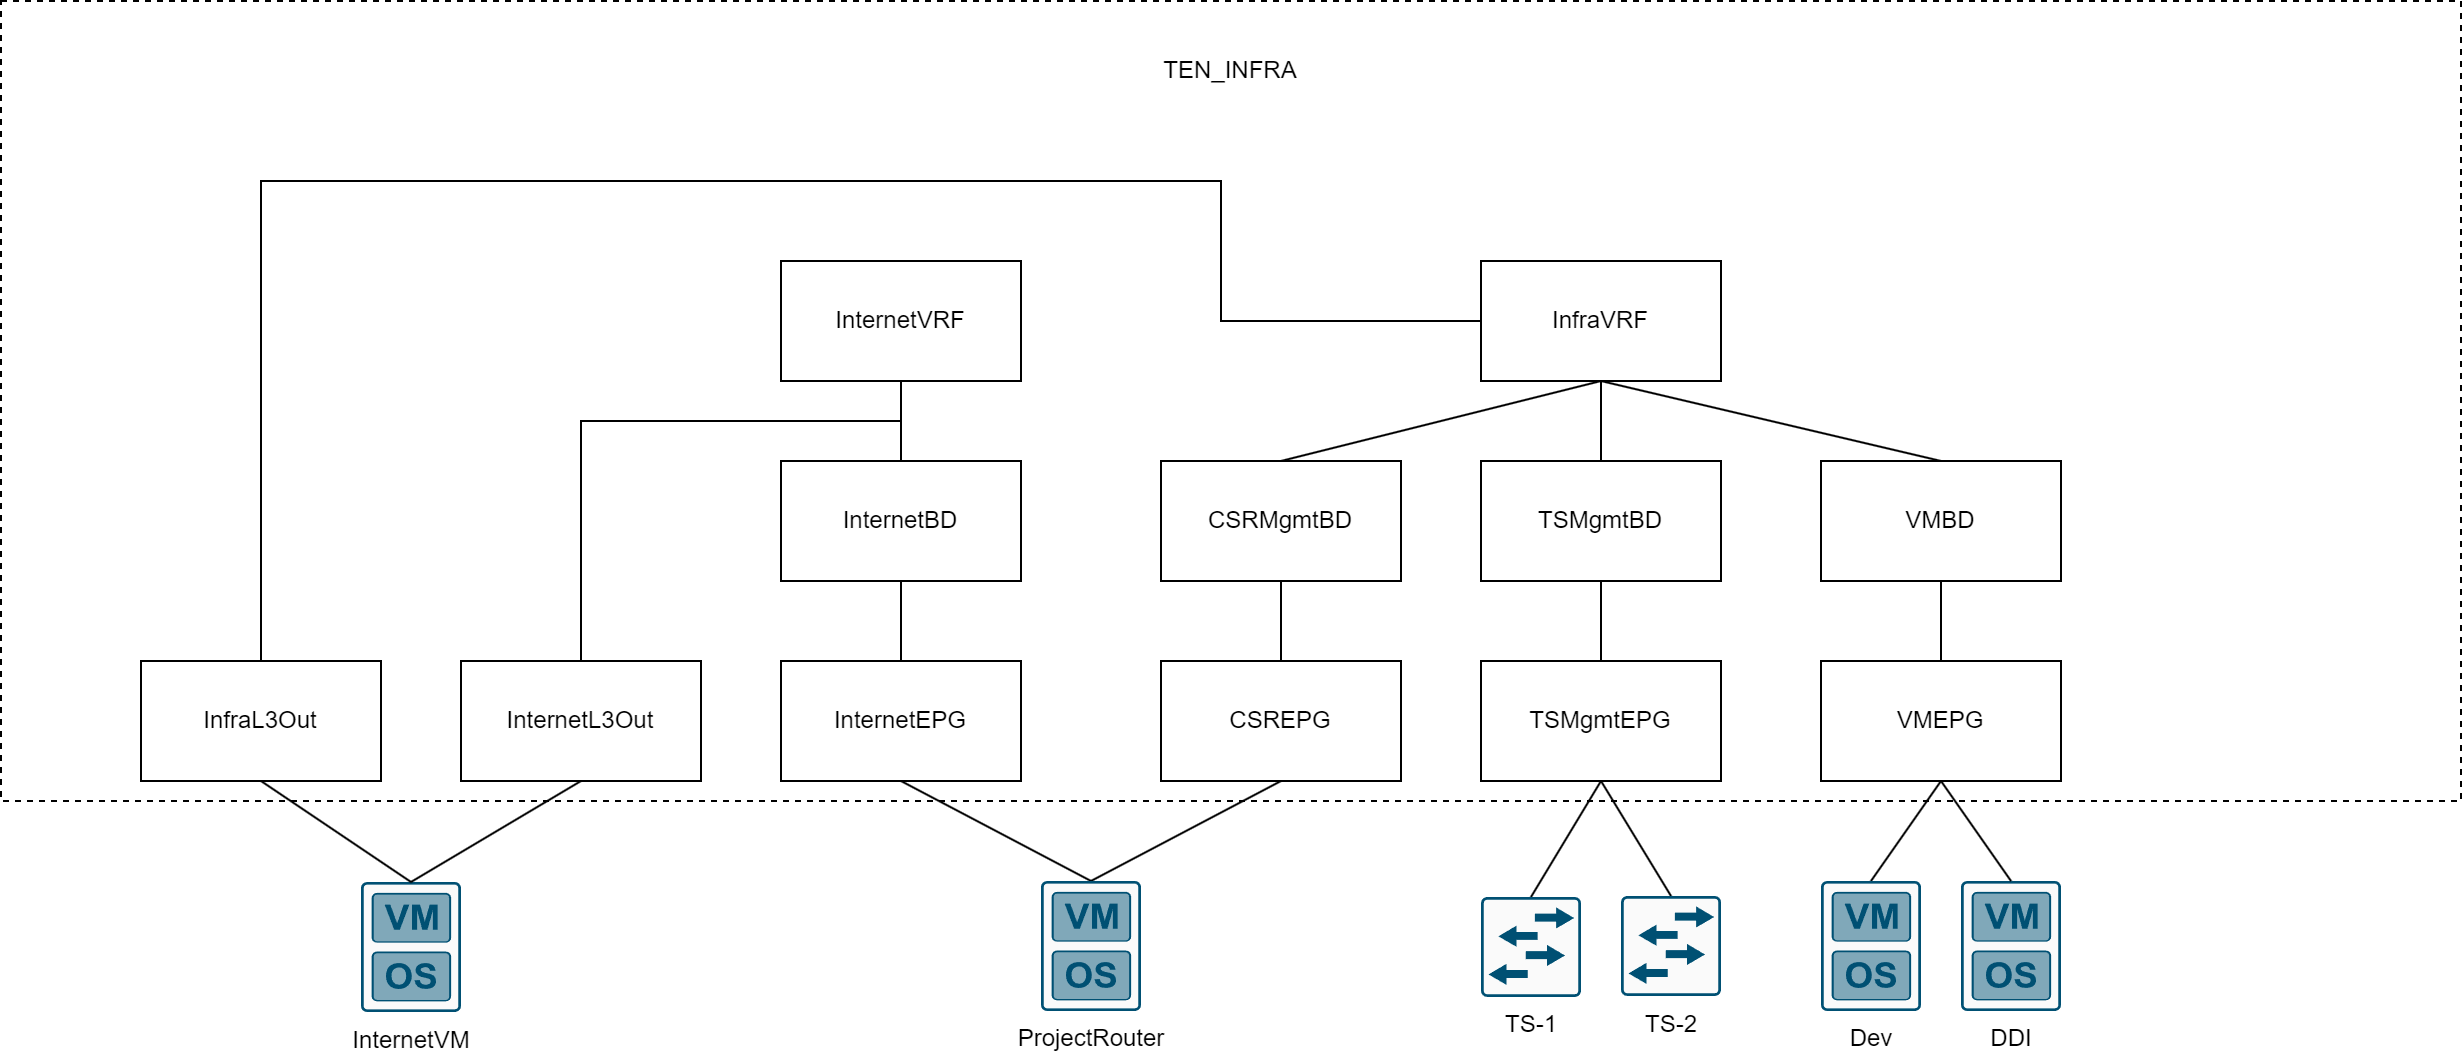
\includegraphics[scale=0.17]{images/epg-topology.png}

    \caption{ACI Policy Overview}
    \label{fig:epg-topology}
\end{figure}

\subsubsection{Infra VRF}
The infra \gls{vrf} will provide L3 routing ability
between all associated bridge domains and \gls{epg}s for the sake of
simplicity, all testbed connectivity for infrastructure will be able to
communicate with one another.

\subsubsection{InfraL3Out}
The InfraL3Out will
be used to advertise connectivity to outside the \gls{aci} fabric. The purpose
of this is to provide internet connectivity via a \gls{nat} router as \gls{aci}
can't provide \gls{nat}. This results in any packets destined for anything
other than locally attached routes present in the InfraVRF will be routed out
of the InfraL3Out.

\gls{ospf} will be used to share routes between \gls{aci}
and the \gls{nat} router.

\subsubsection{Infra Bridge Domains}
Three bridge
domains bring the ability to split connectivity into different subnets and
broadcast domains. This allows for L2 functionality such as DHCP to be easily
controlled and connectivity to be segmented. There will be a bridge domain to
provide connectivity for the following:
\begin{itemize}
    \item Virtual
          Project Routers
          \begin{itemize}
              \item DHCP relay will be
                    operational to forward DHCP discover requests onto the \gls{ddi} server
                    attached to the VM bridge domain, thus allowing newly created VMs to receive an
                    IP address automatically, to facilitate being provisioned by the automation
                    platform.
          \end{itemize}
    \item Terminal Servers
          \begin{itemize}

              \item Allows the automation platform to reach the terminal servers via their
                    RESTCONF \gls{api} to apply the configuration.
          \end{itemize}
    \item
          Infrastructure and testing \gls{vm}s
          \begin{itemize}
              \item Provides
                    connectivity to the fabric for testing and provides services such as DHCP.

          \end{itemize}
\end{itemize}

\subsubsection{Infra EPGs}
Each EPG has a
one-to-one relationship with a bridge domain and is used to provide
connectivity via VMWare \gls{aci} integration and static port associations.

\subsubsection{Internet VRF/BD/EPG}
This \gls{vrf}/\gls{bd}/\gls{epg} will be
used to emulate the project routers having a connection to the internet. This
will be used to test the automation platform's ability to configure the project
routers to have internet connectivity.

Connectivity will be provided via the
InternetL3Out using \gls{ospf} for routing advertisements to the same \gls{nat}
router that provides internet connectivity to the Infra \gls{vrf}, although a
different subnet will be used.

\subsubsection{IP Addressing}
\begin{table}[H]
    \centering
    \begin{tabular}{l l l}
        \hline

        \textbf{Property} & \textbf{Network Address}
                    &
        \textbf{Gateway}
        \\ \hline
        InternetBD  &
        172.16.0.0/24
                    & 172.16.0.254
        \\ \hline

        TSMgmtBD    & 172.16.1.0/24            & 172.16.1.254
        \\ \hline

        CSRMgmtBD   & 172.16.2.0/24            & 172.16.2.254
        \\ \hline

        VMBD        & 172.16.3.0/24            & 172.16.3.254
        \\ \hline
        OOB & 192.168.0.0/24 & 192.168.0.254
    \end{tabular}

    \caption{Functional Requirements}
\end{table}